%!TEX root=../../main.tex


\subsection{Komplexität Aufsetzen}
Systeme wie Galois/Gluon, bei denen man erstmal ewig suchen muss bis man überhaupt einen Guide findet sollten hier schlechter abschneiden. \emph{vorausgesetzt, wir nehmen das hier überhaupt mit auf..}

\subsection{Komplexität eigene Apps schreiben}
Schwierig objektiv zu vergleichen.


\subsection{Pure Performance-Ergebnisse}

\subsection{Ergebnisse Calc time}
\begin{figure}
	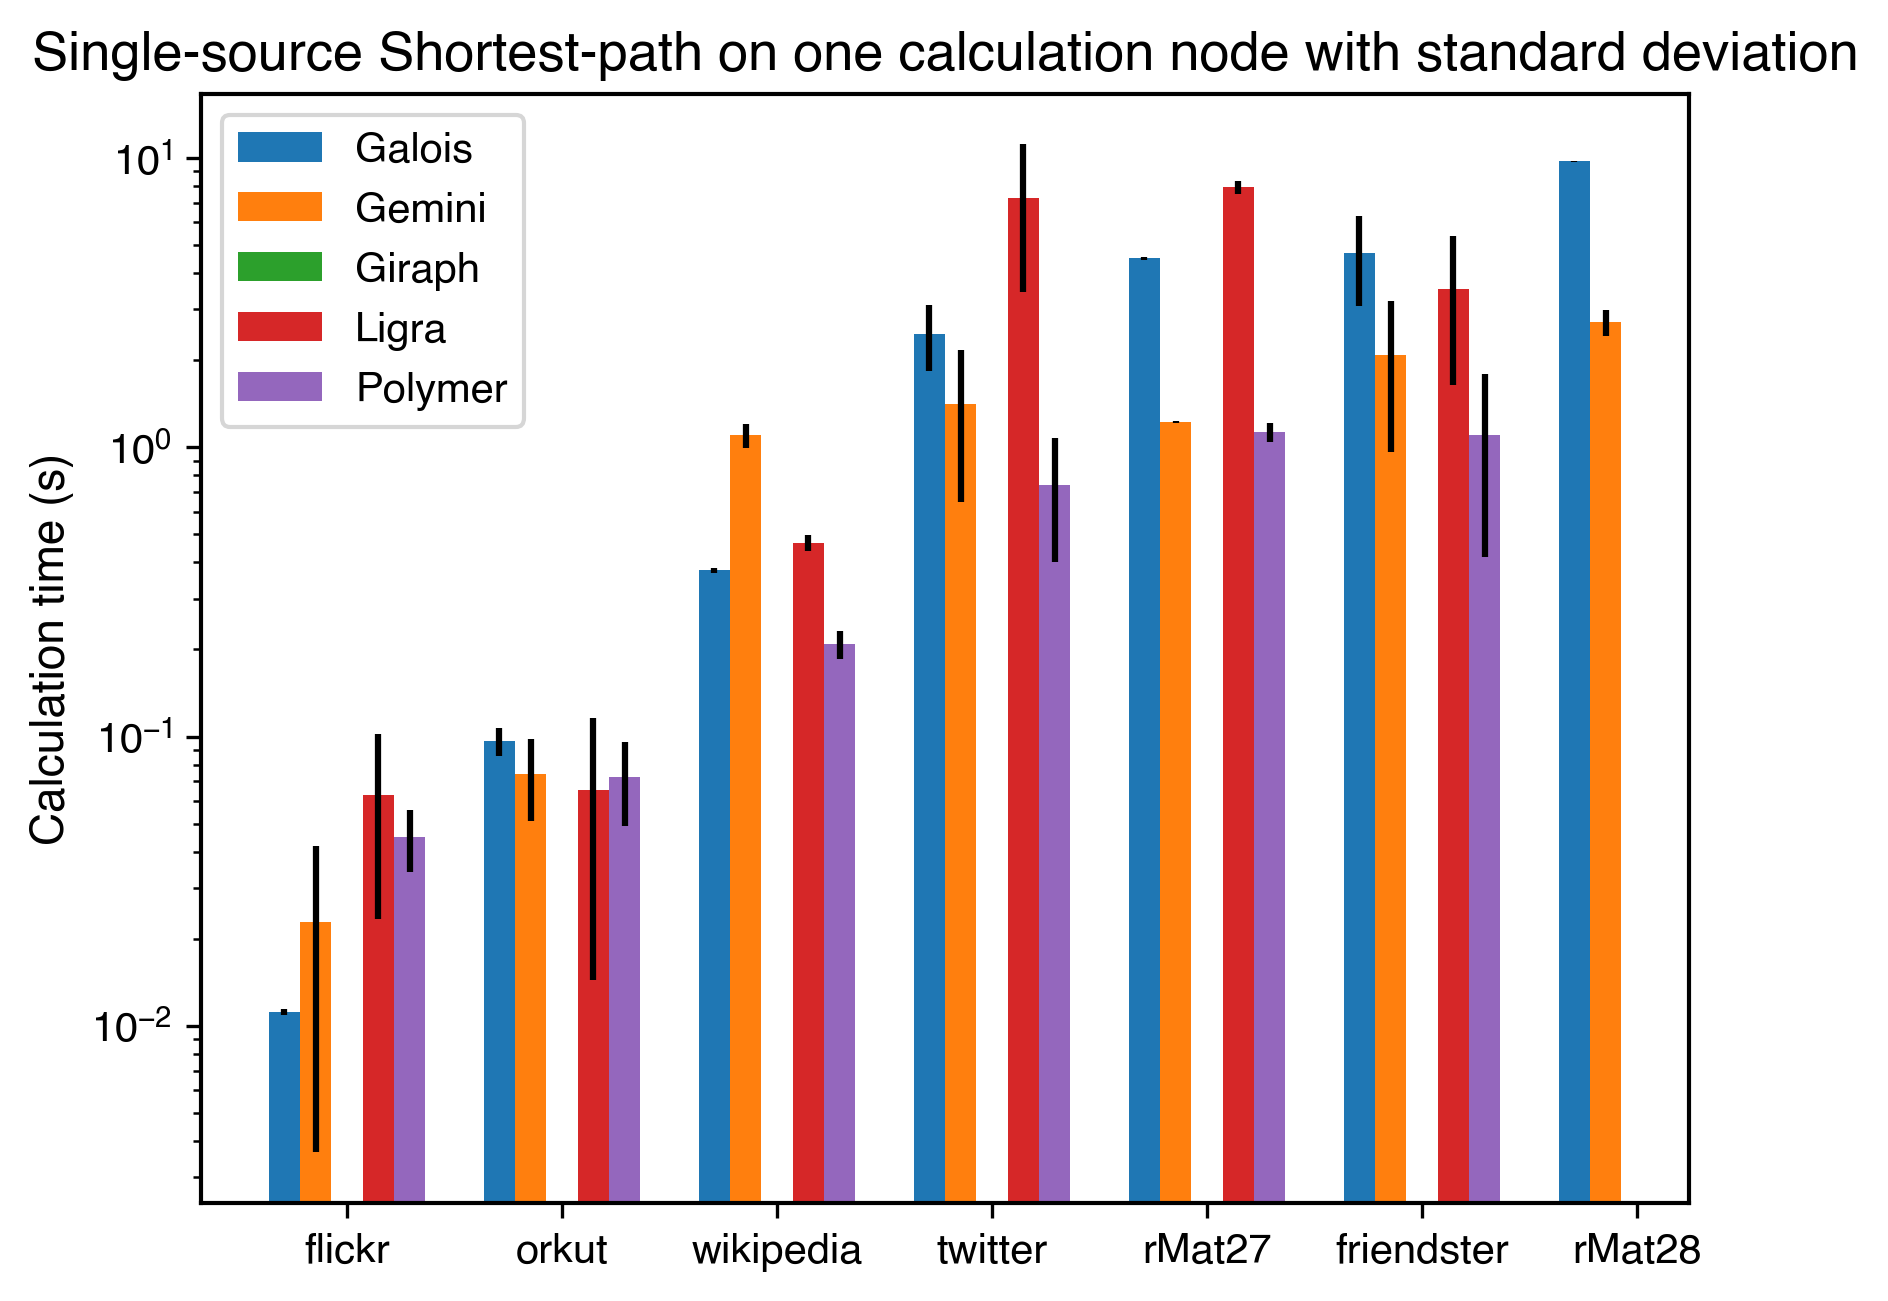
\includegraphics[width=\columnwidth]{../../plots/singleNodeSSSP_calcTime.png}
	\caption{Calculation times for SSSP on a single node}
	\label{fig:singleNodeSSSP_calc}
\end{figure}

\begin{figure}
	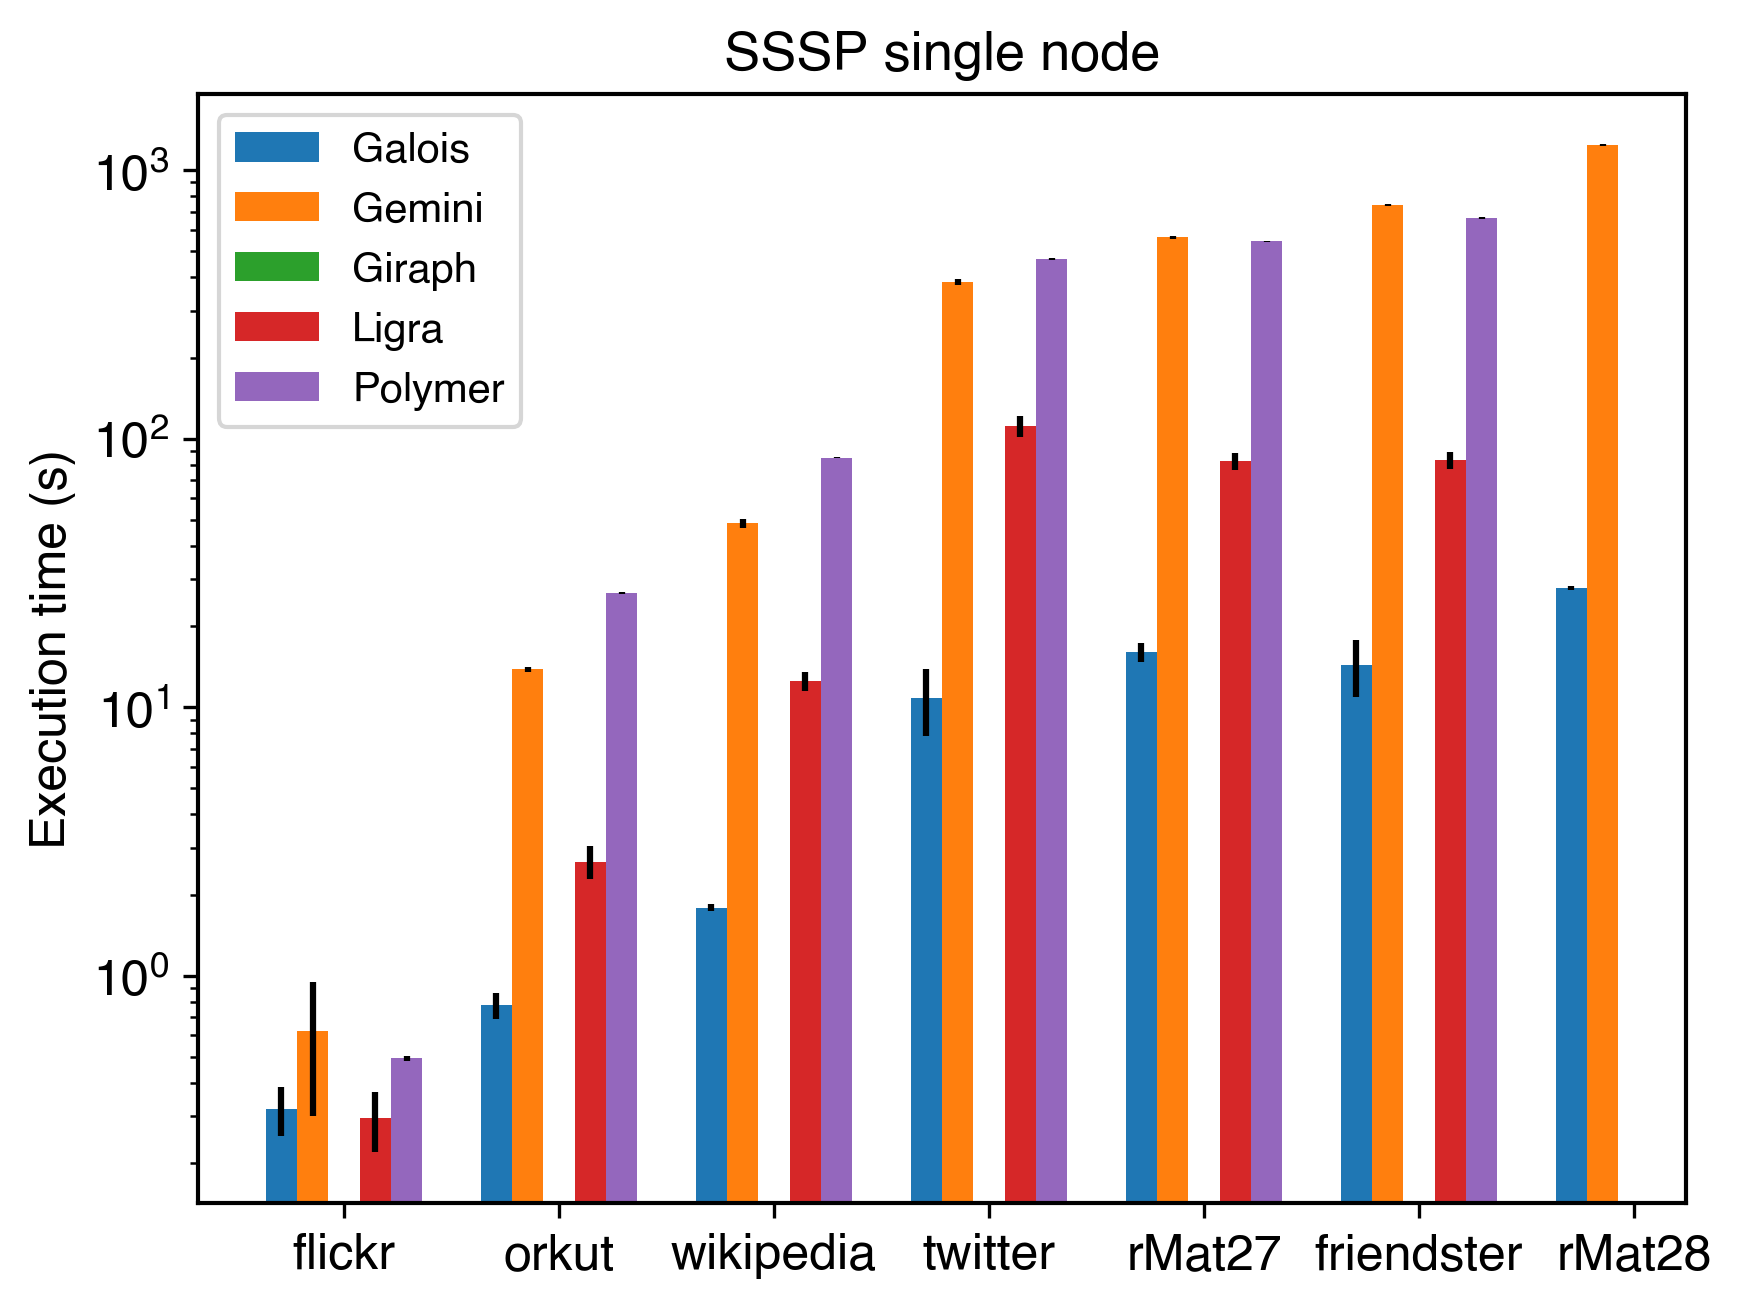
\includegraphics[width=\columnwidth]{../../plots/singleNodeSSSP_execTime.png}
	\caption{Execution times for SSSP on a single node}
	\label{fig:singleNodeSSSP_exec}
\end{figure}


\begin{figure}
	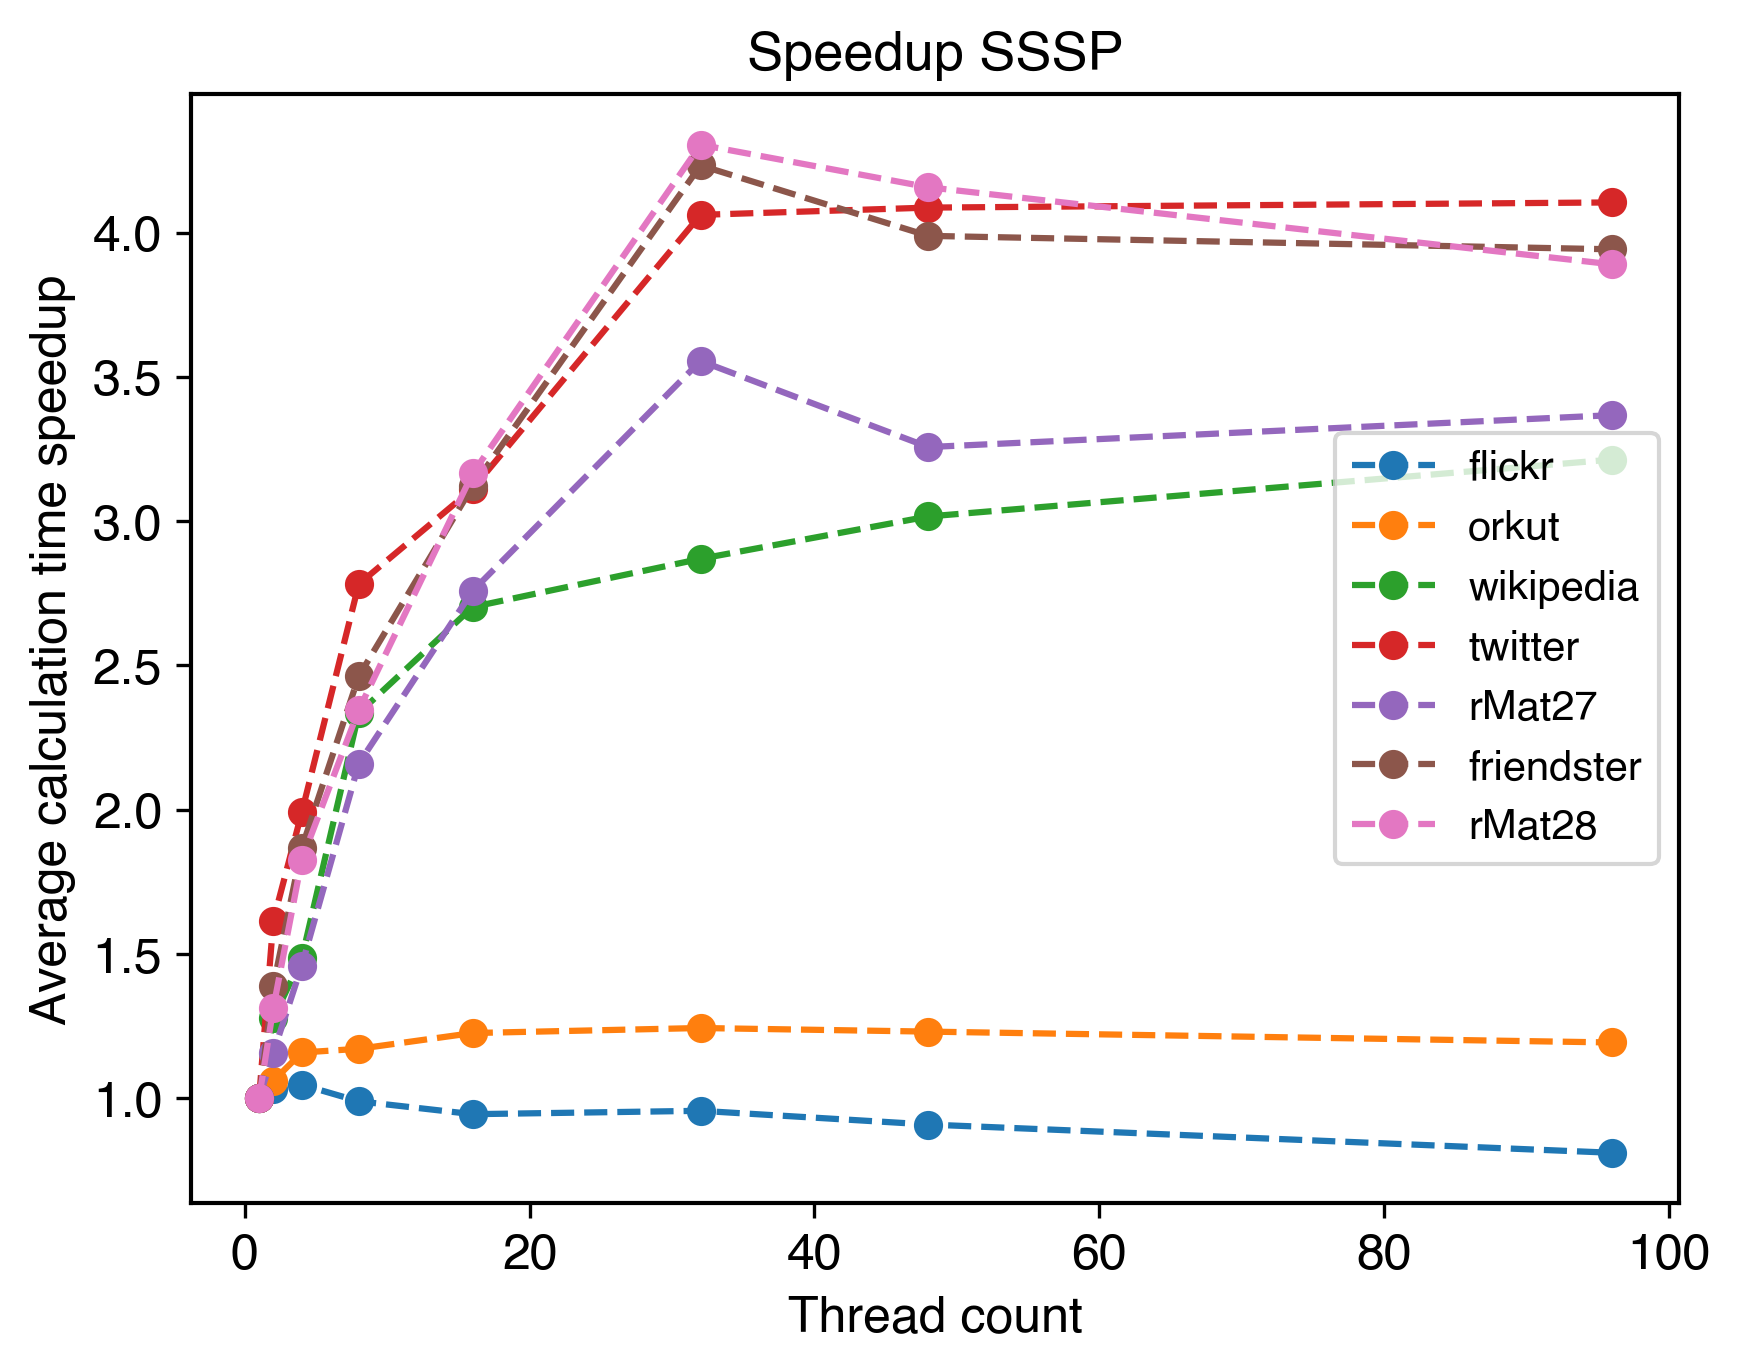
\includegraphics[width=\columnwidth]{../../plots/singleNodeSSSPGaloisThreads.png}
	\caption{Execution times of Galois' SSSP over the thread count}
	\label{fig:singleNodeSSSPGaloisThreads}
\end{figure}
der offensichtliche, wichtige Vergleich

\subsection{Ergebnisse exec time}

hier erhoffe ich mir einen Vergleich der Ladezeiten und erwarte, dass Systeme wie Giraph, die erstmal auf irgendwas warten schlecht abschneiden.
Aber vielleicht ist auch die setup time bei gleichen frameworks zwischen verteilt und shared memory ganz interessant zu vergleichen. 
